% Self-contained "online active loop" schematic — compile with:
%   pdflatex diagram_final.tex
% Output: diagram_final.pdf (single tightly-cropped page).
% No external preamble file; all colors / styles inlined below.

\documentclass[border=10pt]{standalone}
\usepackage{tikz}
\usepackage{amsmath, amssymb}
\usepackage{xcolor}
\usetikzlibrary{shapes.geometric, arrows.meta, positioning, calc}

% ── Palette (subdued, paper-style) ─────────────────────────────────────────
\definecolor{cFill}{HTML}{F4F4F4}      % default block fill (light gray)
\definecolor{cInk}{HTML}{222222}       % nearly-black outlines / text
\definecolor{cMute}{HTML}{777777}      % muted gray
\definecolor{cAccent}{HTML}{2C4A6E}    % single muted dark blue accent
\definecolor{cAccentSoft}{HTML}{C9D3E1}% wash of accent for fills

% ── Reusable styles ────────────────────────────────────────────────────────
\tikzset{
  every node/.style    = {font=\small, text=cInk},
  block/.style         = {rectangle, rounded corners=2pt, draw=cInk, line width=0.5pt,
                          fill=cFill, minimum width=2.8cm, minimum height=0.85cm,
                          align=center, text width=2.6cm, inner sep=4pt},
  focal/.style         = {block, fill=cAccentSoft, draw=cAccent, line width=0.8pt},
  data/.style          = {cylinder, shape border rotate=90, aspect=0.3, draw=cInk,
                          line width=0.5pt, fill=cFill, minimum height=0.8cm,
                          minimum width=1.8cm},
  arrow/.style         = {-Stealth, line width=0.5pt, color=cInk},
  paneltitle/.style    = {font=\bfseries\small, text=cInk},
}

\begin{document}
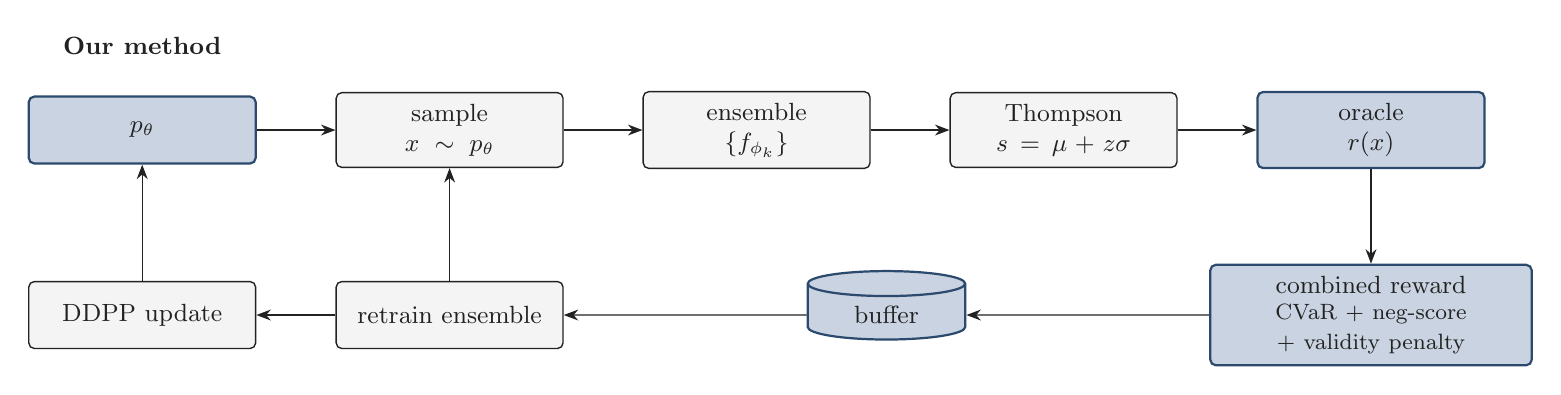
\begin{tikzpicture}[node distance=0.9cm and 1.0cm]

  \node[paneltitle] (title) {Our method};

  % ===== top row =====
  \node[focal, below=0.4cm of title]       (model){$p_\theta$};
  \node[block, right=of model]             (samp) {sample\\$x \sim p_\theta$};
  \node[block, right=of samp]              (ens)  {ensemble\\$\{f_{\phi_k}\}$};
  \node[block, right=of ens]               (ts)   {Thompson\\$s = \mu + z\sigma$};
  \node[focal, right=of ts]                (orac) {oracle\\$r(x)$};

  \draw[arrow] (model) -- (samp);
  \draw[arrow] (samp)  -- (ens);
  \draw[arrow] (ens)   -- (ts);
  \draw[arrow] (ts)    -- (orac);

  % ===== bottom row — all share a single y baseline ===========
  % use combined-reward as the y anchor (the tallest box); place it under oracle
  \node[focal, below=1.2cm of orac, minimum width=4cm, text width=3.8cm]
                                                    (shape) {combined reward\\\footnotesize CVaR + neg-score\\\footnotesize + validity penalty};

  % DDPP update aligned under model, on the same y baseline as `shape`
  \node[block] (ddpp) at (model |- shape) {DDPP update};
  % retrain ensemble aligned under sample
  \node[block] (sur)  at (samp  |- shape) {retrain ensemble};
  % buffer at the x-midpoint of `sur` and `shape`, on the same y baseline
  \coordinate (bufx) at ($(sur.east)!0.5!(shape.west)$);
  \node[data, fill=cAccentSoft, draw=cAccent, line width=0.8pt,
        minimum width=2.0cm, minimum height=0.85cm]
        (buf) at (bufx |- shape) {buffer};

  % horizontal arrows along the bottom row, all on the same baseline
  \draw[arrow] (shape.west) -- (buf.east);
  \draw[arrow] (buf.west)   -- (sur.east);
  \draw[arrow] (sur.west)   -- (ddpp.east);

  % vertical drop from oracle to combined reward
  \draw[arrow] (orac.south) -- (shape.north);

  % vertical feedback up
  \draw[arrow] (sur.north)  -- (samp.south);
  \draw[arrow] (ddpp.north) -- (model.south);

\end{tikzpicture}
\end{document}
